\section{Motivation}
\slides{NI_WS2016_Kap5_RBF}{1}
Datenpunkte als Prototypen der Abbildung $\to$ diese Umkreisen.
\begin{center}
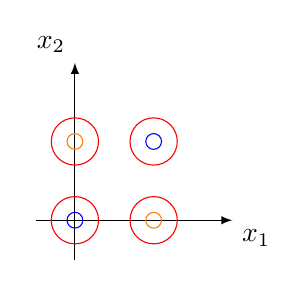
\begin{tikzpicture}[scale=1]
% Koordinatenachsen:
\draw [-latex] (-0.5,0) -- (2,0) node[below right]{$x_1$};
\draw [-latex] (0,-0.5) -- (0,2) node[above left]{$x_2$};
% Funktion:
% Punkte oben:
\draw [orange] (1,0) circle (0.1);
\draw [orange] (0,1) circle (0.1);
\draw [red] (1,0) circle (0.3);
\draw [red] (0,1) circle (0.3);
% Punkte unten
\draw [blue] (1,1) circle (0.1);
\draw [blue] (0,0) circle (0.1);
\draw [red] (1,1) circle (0.3);
\draw [red] (0,0) circle (0.3);
\end{tikzpicture}
\end{center}
Kombiniere die Ausgaben des Netzwerks aus den Ausgaben der Prototyp- bzw. Referenz-Neuronen.\\
Jedes Neuron der Hidden-Schicht bildet einen (Radius von einem) Datenpunkt dar:
\begin{center}
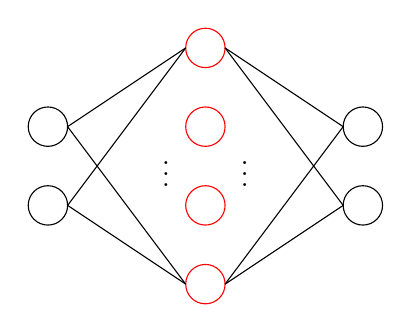
\begin{tikzpicture}[scale=.5]
\draw  (0,1) circle (0.5);
\draw  (0,-1) circle (0.5);

\draw [red] (4,3) circle (0.5);
\draw [red] (4,1) circle (0.5);
\draw [red] (4,-1) circle (0.5);
\draw [red] (4,-3) circle (0.5);

\draw  (8,1) circle (0.5);
\draw  (8,-1) circle (0.5);
\draw (0.5,1) -- (3.5,3);
\draw (0.5,1) -- (3.5,-3);
\draw (0.5,-1) -- (3.5,3);
\draw (0.5,-1) -- (3.5,-3);
\draw (4.5,3) -- (7.5,1) -- (4.5,-3);
\draw (4.5,3) -- (7.5,-1) -- (4.5,-3);
\node at (3,0) {$\vdots$};
\node at (5,0) {$\vdots$};
\end{tikzpicture}
\end{center}
Skalarprodukt:
$$z=\vec{w}^T\cdot \vec{w}$$
Distanzbasierte Aktionsgerade:
$$z=f(\vec{x},\vec{w})$$
$\to$ Vektornormen $\to$ $L_2$-Norm $\to$ $\boxed{z=\sqrt{(x_1-w_1)^2+\ldots + (x_n-w_n)^2}}$ (Euklidischer Abstand) … $z$ als Abstand zwischen $\vec{x}$ und $\vec{w}$.\\
$$y=f(z)\approx e^{-z}$$
$$\boxed{f=\exp \left( -\frac{z^2}{2 \sigma^2} \right)} \text{ Gaußfunktion}$$
\slides{NI_WS2016_Kap5_RBF}{2}
\section{Topologie}
\slides{NI_WS2016_Kap5_RBF}{3}
\section{Berechnungsvorschriften}
\slides{NI_WS2016_Kap5_RBF}{4}
\slides{NI_WS2016_Kap5_RBF}{5}
\section{Trainingsregime}
\slides{NI_WS2016_Kap5_RBF}{6}

\subsection{Bestimmung der Gewichte von der Eingangs- zur RBF-Schicht}
\slides{NI_WS2016_Kap5_RBF}{7}
\slides{NI_WS2016_Kap5_RBF}{8}

\subsection{Bestimmung der Varianzen}
\slides{NI_WS2016_Kap5_RBF}{9}
\slides{NI_WS2016_Kap5_RBF}{10}

\subsection{Bestimmung der Gewichte von der RBF- zur Ausgabeschicht}
\slides{NI_WS2016_Kap5_RBF}{11}
$\vec{A}=f(\vec{X}, \vec{W}, \vec{\sigma})$
\slides{NI_WS2016_Kap5_RBF}{12}
Achtung bei Inverser: Elemente dürfen nicht linear abhängig sein!

\subsection{Iteratives Nachtraining}
\slides{NI_WS2016_Kap5_RBF}{13}

\subsection{Weitere mathematische Betrachtungen}
\slides{NI_WS2016_Kap5_RBF}{14}






